\documentclass[10pt,a4paper]{article}

%%%%%%%%%%%%%%%%%%%%%%%%%%%
% MODIFY:

\newcommand{\authorA}{ALEX PASQUALI (03754113)}
\newcommand{\authorB}{NICOLA GUGOLE (03753996)}
\newcommand{\groupNumber}{A} % - YOUR GROUP
\newcommand{\exerciseNumber}{5} % - THE NUMBER OF THE EXERCISE
\newcommand{\sourceCodeLink}{\url{https://github.com/AlexPasqua/MLCMS-exercises}}

\newcommand{\workPerAuthor}{
\authorA&Task 1&50\%\\
      &Task 2&50\%\\
      &Task 3&50\%\\
      &Task 4&50\%\\
      &Task 5&50\%\\
      \hline
\authorB&Task 1&50\%\\
      &Task 2&50\%\\
      &Task 3&50\%\\
      &Task 4&50\%\\
      &Task 5&50\%\\
}

%%%%%%%%%%%%%%%%%%%%%%%%%%%

%%
% imports for the exercise sheets
%

\usepackage[utf8]{inputenc}
\usepackage{amsmath}
\usepackage{amsfonts}
\usepackage{amssymb}

\usepackage[yyyymmdd]{datetime}
\renewcommand{\dateseparator}{--}

\usepackage[left=2cm,right=2cm,top=3cm,bottom=3cm]{geometry}

\usepackage{hyperref}

\usepackage{amsthm}
\newtheorem{lem}{Lemma}
\newtheorem{thm}{Theorem}
\newtheorem{cor}{Corollary}
\newtheorem{rem}{Remark}
\newtheorem{definition}{Definition}
\newtheorem{ter}{Terminology}

\usepackage{graphicx}

\newcommand{\M}{\mathcal{M}}
\newcommand{\N}{\mathcal{N}}
\newcommand{\K}{\mathcal{K}}
\newcommand{\SPDk}{\mathbb{P}^k}
\newcommand{\vol}{\text{vol}}

\newcommand{\Figref}[1]{Figure~\ref{#1}}
\newcommand{\figref}[1]{figure~\ref{#1}}
\newcommand{\Eqnref}[1]{Equation~(\eqref{#1})}
\newcommand{\eqnref}[1]{equation~(\eqref{#1})}

\usepackage{float}
\usepackage{tabularx}

\usepackage{fancyhdr}
\pagestyle{fancy}

\usepackage{totcount}
\newtotcounter{taskCounter}
\newtotcounter{pointCounter}
\newenvironment{task}[1]{\noindent\stepcounter{taskCounter}\textbf{Report on task #1}\smallbreak\hrule\smallbreak}{\smallbreak\hrule\bigbreak}


\title{Report for exercise \exerciseNumber~from group~\groupNumber}

\makeatletter
\let\thetitle\@title
\let\theauthor\@author
\let\thedate\@date
\makeatother

\providecommand{\versiondate}{\today}

\lhead{Exercise sheet \exerciseNumber}
\chead{Master Praktikum: Modelling and Simulation of Crowds WS2019/20}
\rhead{TUM}
\lfoot{Report of Group \groupNumber}
\cfoot{\thepage}
\rfoot{Last compiled: \versiondate}
\renewcommand{\headrulewidth}{0.4pt}
\renewcommand{\footrulewidth}{0.4pt}

\newcommand{\frontpage}{
\begin{center}
\textbf{\thetitle}\\~\\
\end{center}
\begin{table}[H]
\begin{tabular}{ll}
Tasks addressed:&\total{taskCounter}\\
Authors:&\authorA\\
&\authorB\\
&\authorC\\
Last compiled:&\versiondate\\
Source code:&\sourceCodeLink
\end{tabular}
\end{table}
\vfill
The work on tasks was divided in the following way:
\begin{table}[H]
\begin{tabularx}{\textwidth}{X|p{2cm}|p{2cm}}
\workPerAuthor
\end{tabularx}
\end{table}
\newpage
}

\begin{document}

\frontpage

\begin{task}{1, Approximating functions}
This task consists in approximating linear and non-linear functions.
We creatd a Python script called \texttt{function\_approximation.py} that contains a series of functions to read the data, compute the radial basis functions, approximate linear and non linear data and plot the approximated function over the actual data.

\paragraph{Part 1}
This part consists in linearly approximating the linear data contained in \texttt{linear\_function\_data.txt}.
To accomplish the task, in \texttt{function\_approximation.py}, we created the function \texttt{approx\_lin\_func} as a sort of wrapper for numpy's least squares solver (\texttt{numpy.linalg.lstsq}): it simply splits the data into points and targets (if the path is provided instead of the actual data, the function reads the file first), then it applies numpy's solver and returns the result.
The code is shown in Figure \ref{fig:approx-lin-func}, while the plot of the approximated function over the actual data is instead shown in Figure \ref{fig:approximated-func-over-linear-data}, where, as expected, it is possible to see that the data is approximated very well.
Using the radial basis functions to approximate linear data is not the best idea because, to reach a semi-decent approximation, we should use a number of basis functions near to the number of points (more is not possible, because we would need more centers than actual points) and a large $\epsilon$.
This is shown in Figure \ref{fig:approximated-func-over-linear-data}.

\begin{figure}[H]
    \centering
    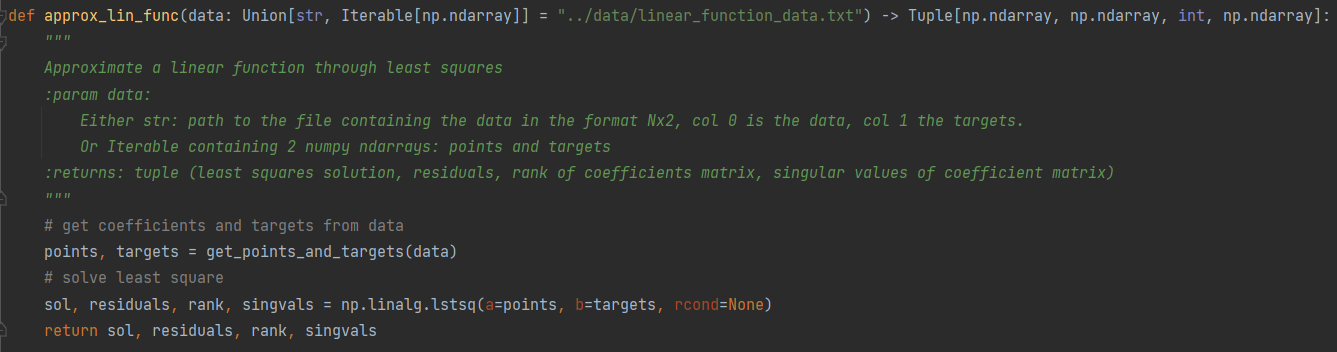
\includegraphics[width=1.0\textwidth]{images/approx_lin_func.png}
    \caption{Function to approximate linear data.}
    \label{fig:approx-lin-func}
\end{figure}

\begin{figure}[H]
    \centering
    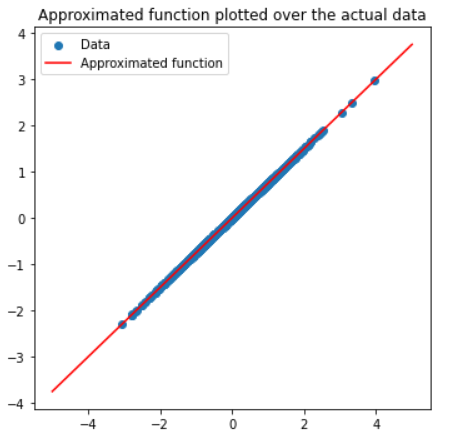
\includegraphics[scale=0.8]{images/plot_approximated_func_over_linear_data.png}
    \caption{Plot of the linearly approximated function over the actual linear data contained in the file \texttt{linear\_function\_data.txt}.}
    \label{fig:approximated-func-over-linear-data}
\end{figure}

\begin{figure}[H]
    \centering
    \subfloats[a]{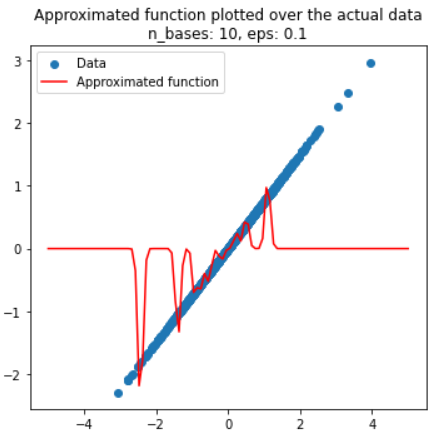
\includegraphics[width=0.45\textwidth]{images/linear_data_approx_with_bases.png}}
    \hfill
    \subfloats[b]{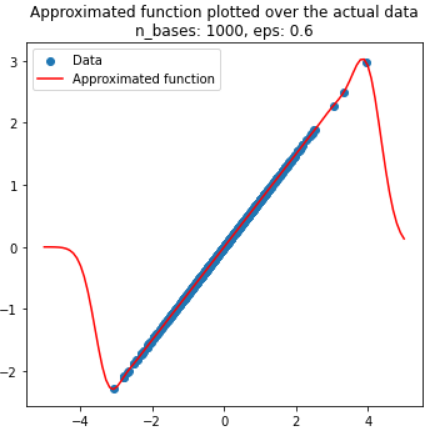
\includegraphics[width=0.45\textwidth]{images/linear_data_approx_with_bases_2.png}}
    \caption{Approximation of linear data with a combination of radial basis functions.}
    \label{fig:approximated-func-over-linear-data}
\end{figure}

\paragraph{Part 2}
The second part consists of performing again a linear approximation, but this time the data, contained in \texttt{nonlinear\-function\_data.txt}, is non-linear (as the name of the file suggests).
The procedure is the same as for part 1, we simply change the path to the data file.
The plot of the approximated function over the data is shown in Figure \ref{fig:linearly-approximated-func-over-nonlinear-data}, and, as expected, approximating such data with a straight line does not provide good results.

\begin{figure}[H]
    \centering
    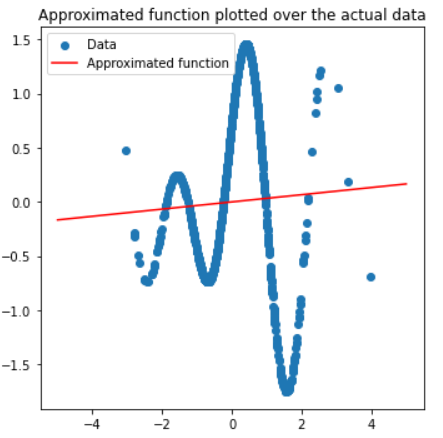
\includegraphics[scale=0.8]{images/plot_linearly_approximated_func_over_nonlinear_data.png}
    \caption{Plot of the linearly approximated function over the actual non-linear data contained in the file \texttt{nonlinear\_function\_data.txt}.}
    \label{fig:linearly-approximated-func-over-nonlinear-data}
\end{figure}

\paragraph{Part 3}
This time the non-linear data (again the one in \texttt{nonlinear\_function\_data.txt}) is approximated as in Eq. \ref{eq:approx-with-radial-basis} with a combination of radial basis functions having the form showed in Eq. \ref{eq:radial-basis}.

\begin{equation}\label{eq:approx-with-radial-basis}
    f(x) = \sum_{l=1}^L c_l \phi_l(x)
\end{equation}

\begin{equation}\label{eq:radial-basis}
    \phi_l(x) = \exp \left(- \frac{\|x_l - x\|^2}{\epsilon^2}\right)
\end{equation}

where $x_l$ is the center point of the function, chosen randomly among the data points, and $\epsilon$ indicates how wide the Gaussian is.\\
We implemented a function called \texttt{approx\_nonlin\_func} (Fig. \ref{fig:approx-nonlin-func}) and tried different combination for the values of $\epsilon$ and $L$ (i.e. the number of basis functions used for the approximation), which are reported in Table \ref{tab:eps-L}.
Obviously, a value of 12 for $\epsilon$ is way bigger than needed, but it provides an insight about the behavior of the basis functions when this parameter grows a lot.
Figure \ref{fig:bases-eps} shows how adding more functions is in general a good thing, but of course the approximation gets more costly to compute.
The value of $\epsilon$ is very important as well, in fact, with the same number of functions, the results can be pretty different.
This can be observed in Figure \ref{fig:bases-eps}, looking at how different the approximation is between the plots on the same row (that correspond to different values of $\epsilon$, but with the same number of functions).
Finally, in Figure \hyperref[fig:bases-eps]{\ref{fig:bases-eps}(e)}
it is shown an example of what a too large value of $\epsilon$ can do.

\begin{figure}[H]
    \centering
    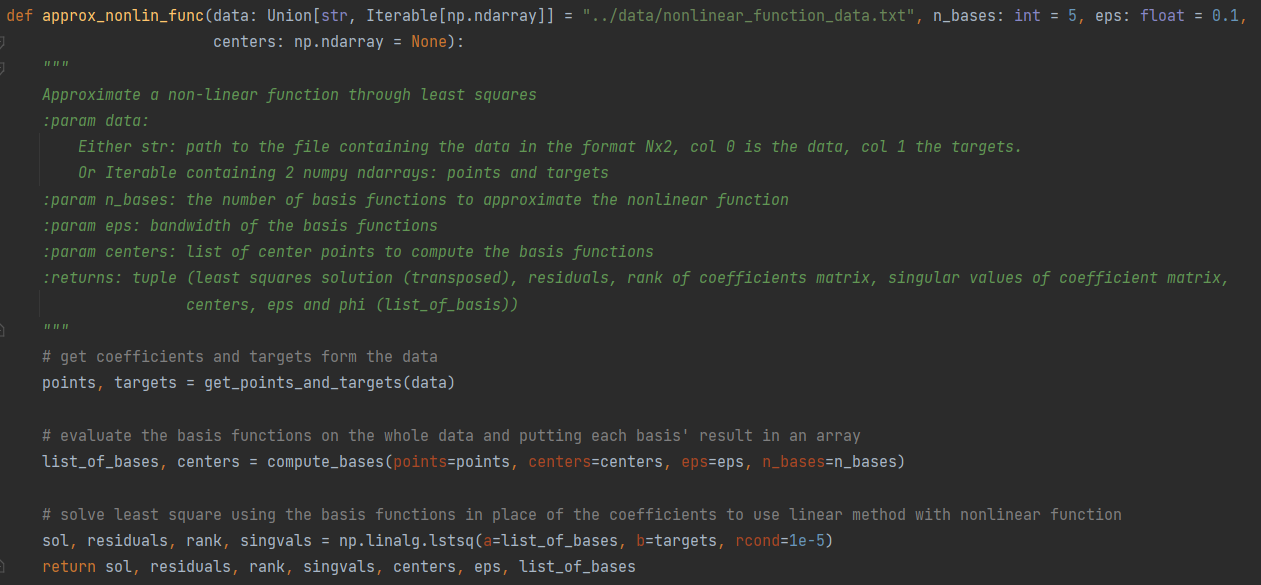
\includegraphics[width=1.0\textwidth]{images/approx_nonlin_func.png}
    \caption{Code of the function \texttt{approx\_nonlin\_func} implementing a function approximation through a combination of radial basis functions.}
    \label{fig:approx-nonlin-func}
\end{figure}

\begin{table}[H]
    \centering
    \begin{tabular}{|c|c|}
        \hline
        \textbf{Parameter} & \textbf{Values}\\
        \hline
        $\epsilon$ & 0.1, 0.2, 0.5, 0.8, 12\\
        $L$ & 3, 5, 8, 10\\
        \hline
    \end{tabular}
    \caption{Values tested for $\epsilon$ and $L$.}
    \label{tab:eps-L}
\end{table}

\begin{figure}[H]
    \centering
    \subfloat[a]{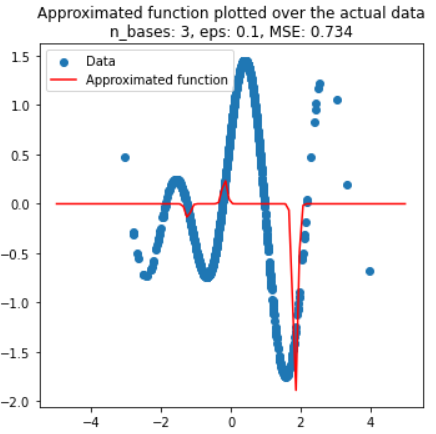
\includegraphics[width=0.44\textwidth]{images/bases3_eps0.1.png}}
    \hfill
    \subfloat[b]{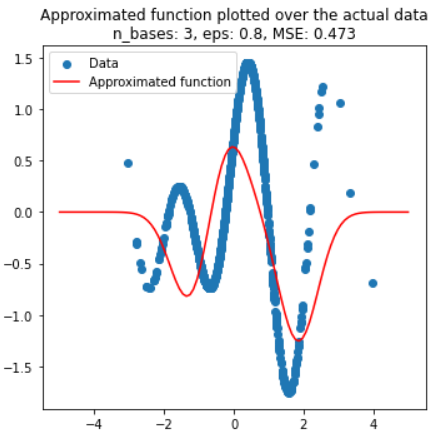
\includegraphics[width=0.44\textwidth]{images/bases3_eps0.8.png}}
    \subfloat[c]{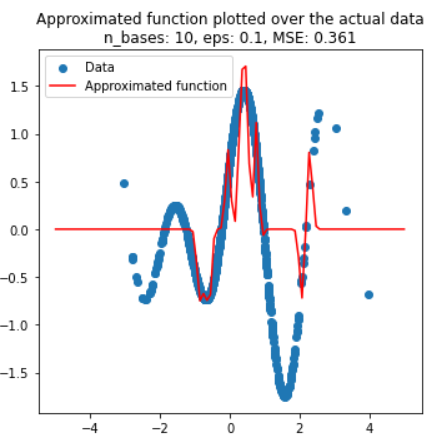
\includegraphics[width=0.44\textwidth]{images/bases10_eps0.1.png}}
    \hfill
    \subfloat[d]{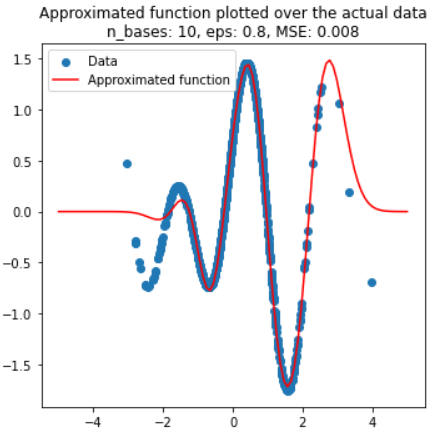
\includegraphics[width=0.44\textwidth]{images/bases10_eps0.8.png}}
    \subfloat[e]{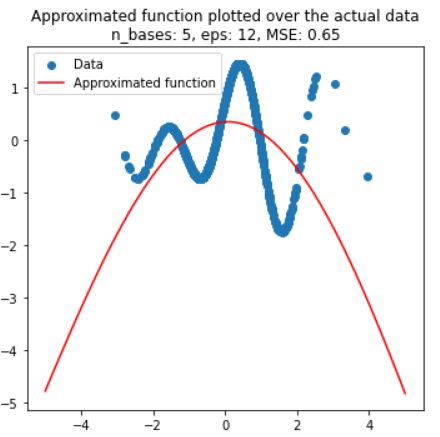
\includegraphics[width=0.44\textwidth]{images/bases5_eps12.png}}
    \caption{Examples of approximations of the non-linear data (contained in \texttt{nonlinear\_function\_data.txt}) with a varying number of radial basis functions and a varying $\epsilon$.}
    \label{fig:bases-eps}
\end{figure}

\end{task}


\begin{task}{2, Approximating linear vector fields}
This task is centered around approximating a given 2 dimensional \textit{linear vectorfield data}. In particular we are given two instants in time for the dataset, \texttt{x0} and \texttt{x1}, with points in \texttt{x0} reaching \texttt{x1} after a certain unknown $\Delta t$ (although from the task text we know the value should be \textbf{0.1}).\\
\paragraph{Part 1}
\begin{figure}[H]
    \centering
    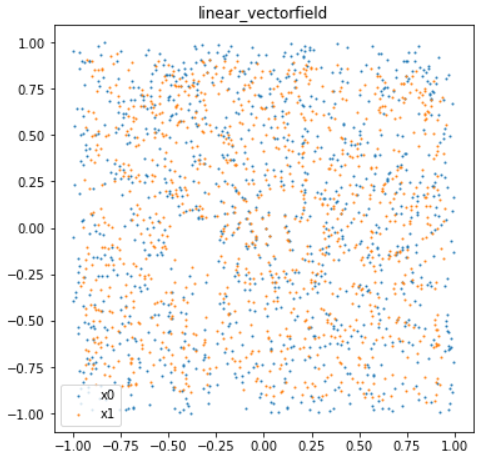
\includegraphics[scale=0.5]{images/task2_data.png}
    \caption{linear vectorfield dataset}
    \label{fig:t2-data}
\end{figure}
The first part of \textit{task 2} asks to estimate the linear vector field \texttt{v} that leads from \texttt{x0} to \texttt{x1} such that the MSE error will be minimized in part 2, regarding a trajectory simulation with $\Delta t = 0.1$. With that \texttt{v} we can then approximate the matrix \texttt{A} solving a least square problem using \texttt{x0} and \texttt{v}. 

To search for such an optimal $\Delta t$ we decided to test 500 possibilities in an interval ranging from 0.0001 to 0.5, basically approximating \texttt{v}, creating \texttt{A} and then simulating the trajectory to generate \texttt{x1} to be able to assess the MSE. We decided to use \texttt{solve\_ivp} from \texttt{scipy.integrate} as numerical solver. \textbf{\hyperref[fig:t2-attempts]{Figure \ref{fig:t2-attempts}}} shows a little part of the search, which winner was $\Delta t = 0.14336$ with an MSE equal to \textbf{0.0026804}. Such a difference between the winning $\Delta t$ and the forecasted one (0.1) was explained in the Q&A as a derivative of having such an approximation in calculating \texttt{v}. 
\begin{figure}[H]
    \centering
    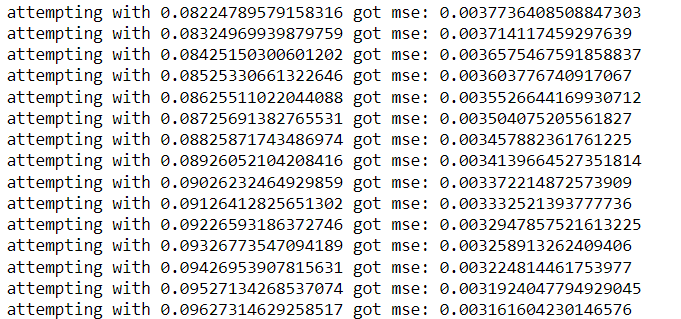
\includegraphics[scale=0.5]{images/task2_attempts.png}
    \caption{small section of trying different \texttt{dt} searching for lowest MSE value}
    \label{fig:t2-attempts}
\end{figure}
\paragraph{Part 2}
This part of the task asks to estimate \texttt{A} with the chosen $\Delta t$ to then solve the linear system up to a $T_{end} = 0.1$ and calculate once again the MSE. The MSE is exactly the one written before since the optimal $\Delta t$ was already discussed and utilized to estimate \texttt{A}. In \textbf{\hyperref[fig:task2-traj]{Figure \ref{fig:task2-traj}}} one can appreciate in orange the trajectories that are moving all the initial points \texttt{x0} nearer to the objective points \texttt{x1} (in blue). The residual error above the image shows how the found \texttt{A} is a good approximation.
\begin{figure}[H]
    \centering
    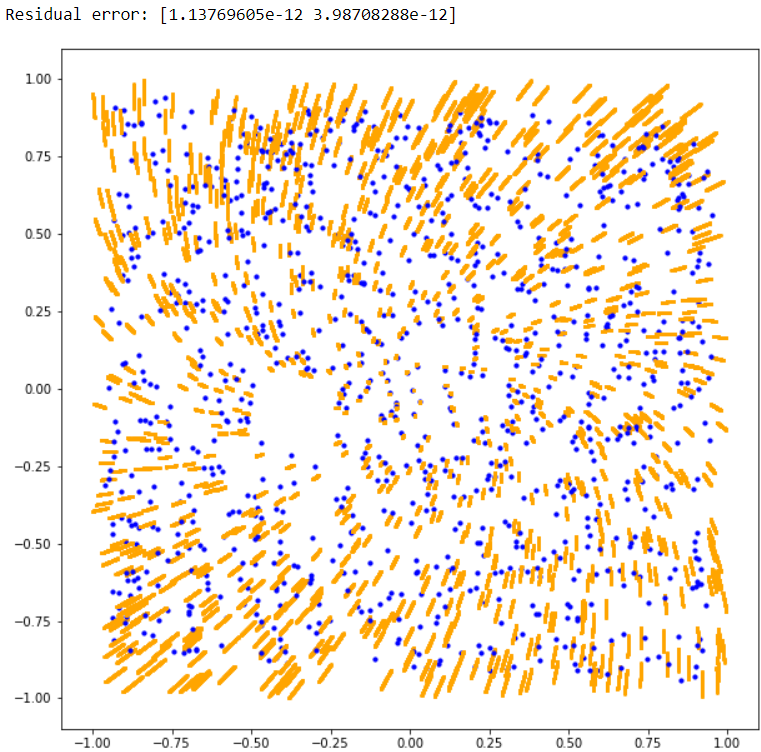
\includegraphics[scale=0.5]{images/task2_part2.png}
    \caption{trajectory simulation from \texttt{x0} (in orange) lasting $\Delta t = 0.1$, with \texttt{x1} scattered (in blue)}
    \label{fig:task2-traj}
\end{figure}
\paragraph{Part 3} the final part of the task is graphically explained by \textbf{\hyperref[fig:task2-portrait]{Figure \ref{fig:task2-portrait}}}, where the phase portrait of the linear vector field is shown. It is clear to see how the dynamical system locally has a single attractive steady in the origin. 

This part of the task is in particular asking to choose a point far away from the initial data, such as \texttt{(10,10)} and to solve its trajectory  for a long time, $T_{end} = 100$. This fact is shown in the figure by the orange scatter plot, where the far apart point can be seen reaching at big leaps the steady state in the origin, confirming the phase portrait of the vector field.
\begin{figure}[H]
    \centering
    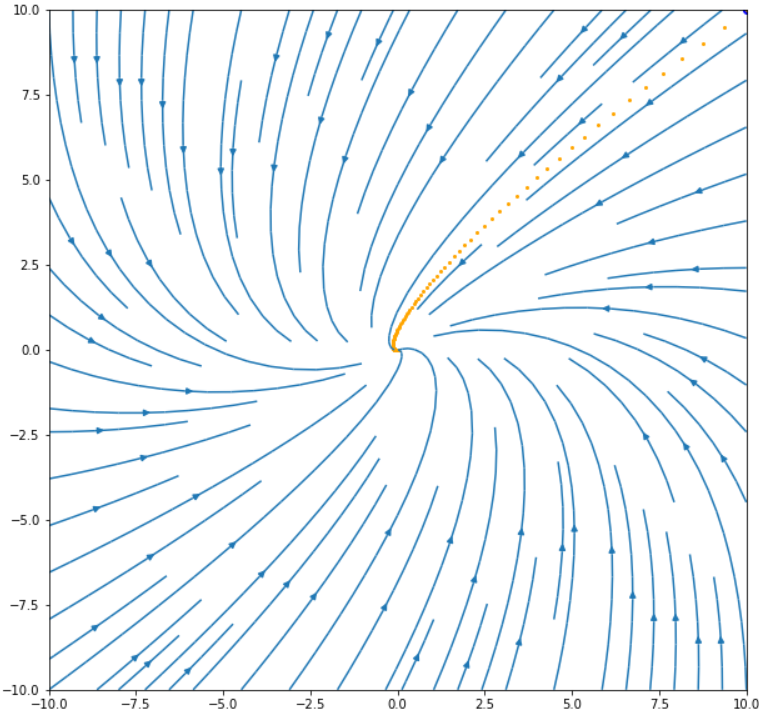
\includegraphics[scale=0.5]{images/task2_part3.png}
    \caption{phase portrait of linearly approximated vector field - trajectory of point with \texttt{x0 = [10,10]}}
    \label{fig:task2-portrait}
\end{figure}
\end{task}


\begin{task}{3, Approximating nonlinear vector fields}
This task revolves around working on a given \textit{nonlinear vector field dataset} composed once again of two moments in time, starting points \texttt{x0} and points \texttt{x1} after an unknown $\Delta t$.  
\begin{figure}[H]
    \centering
    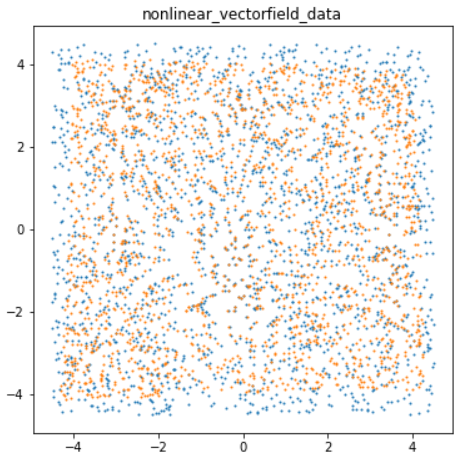
\includegraphics[scale=0.5]{images/task3_data.png}
    \caption{non linear vectorfield dataset}
    \label{fig:task3-data}
\end{figure}
\paragraph{Part 1}
Firstly we are asked to estimate the vector field with a linear operator, as we did in the previous task for the \textit{linear vector field dataset}. We therefore fixed a \texttt{dt} (to 0.1) to approximate \texttt{v} using again the finite difference formula. With the approximation we linearly estimated \texttt{A} (with a residual error of \texttt{[3890.04548426 3563.97075073]} and we simulated the system up to time \textbf{0.5}, finding out that, at end time, the MSE has a value equal to \textbf{0.201521}, while the moment where the system got closer (starting from \texttt{x0}) to \texttt{x1} was at \texttt{t = 0.101010}, with an MSE of \textbf{0.037288}. This shows that the initial choice of \texttt{dt} influences the moment where the system gets closer to \texttt{x1}, as also the choice of \texttt{dt} changed accordingly the time with best (lowest) MSE. \textbf{\hyperref[fig:task3-linportrait]{Figure \ref{fig:task3-linportrait}}} shows the phase portrait for the linearly estimated vector field, showing a system resembling a \textit{stable node}, with a single steady state that appears to be in the origin.
\begin{figure}[H]
    \centering
    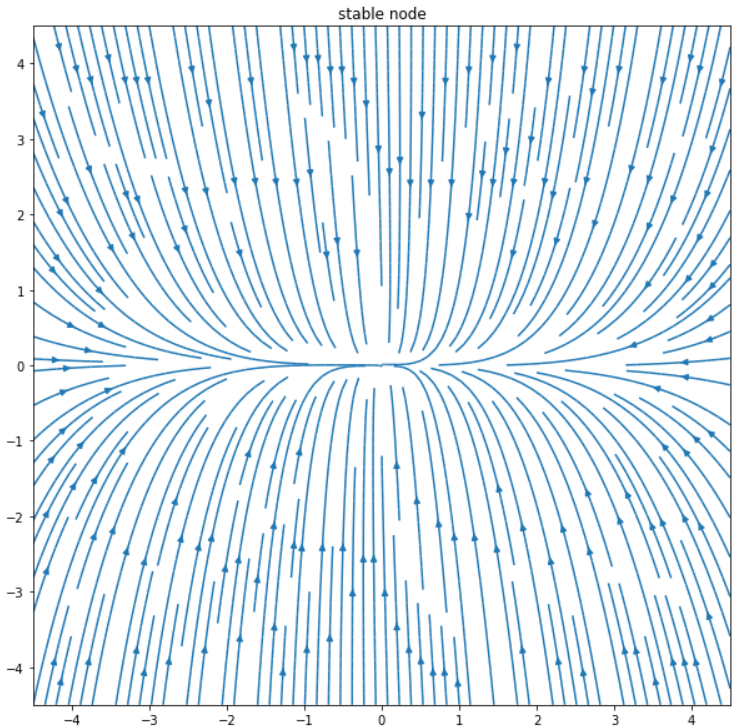
\includegraphics[scale=0.5]{images/task3-linportrait.png}
    \caption{phase portrait of linear approximation for the \textit{non linear vector field dataset}}
    \label{fig:task3-linportrait}
\end{figure}

\paragraph{Part 2}
After trying to linearly approximate the vector field, we are asked to approximate it non-linearly, using the same \textbf{RBF} function we described before. To find the best parameters, we applied a grid search through the method \texttt{find\_best\_rbf\_configuration}, trying different values for \texttt{eps} (0.3, 0.5, 0.7, 1.0, 5.0, 10.0, 20.0) and for \texttt{n\_bases} (trying 20 equally spaced bases numbers between 100 and 1000). To assert the best parameters we performed MSE analysis on each of the configurations, searching for the lowest MSE one can encounter during the trajectory generation of a particular configuration. After trying the process for some times we noticed the best number of bases slightly changed from time to time (probably due to a change of the center points of the radial basis functions), revolving around \textbf{500} most of the times, but keeping \texttt{eps = 5.0}. Reporting here the final execution results, the best parameters were:
\begin{itemize}
    \item \texttt{n\_bases}: 479 
    \item \texttt{eps}: 5.0
    \item \texttt{best dt}: 0.11 (once again approximating the chosen \texttt{dt})
\end{itemize}
The best performing non-linear approximation gives a much better MSE, going down to \textbf{0.000314}, showing how this method greatly outperforms the linear counterpart. This is immediately visually clear by comparing the final trajectory points using the best linear approximation and the best non-linear approximation, as reported in \textbf{\hyperref[fig:task3-linvsnonlin]{Figure \ref{fig:task3-linvsnonlin}}}. Therefore one can conclude that the non linear approximation leads to a much nearer solution with respect to the linear approximation, therefore leading to the vector field itself being non linear.

\begin{figure}[ht!]
 \centering
 
 \subfloat{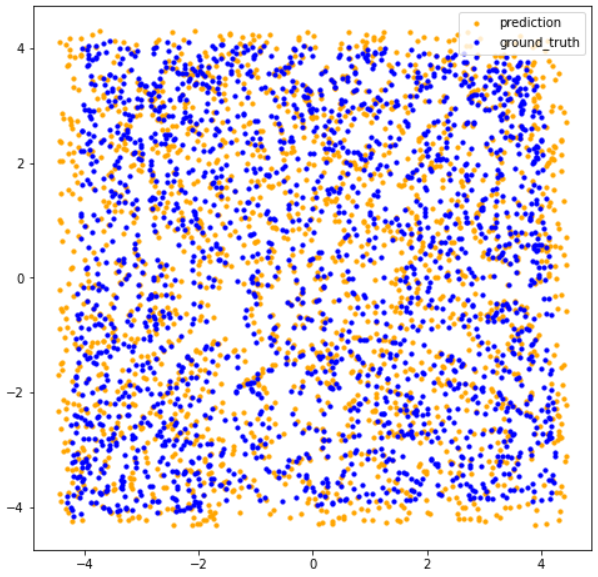
\includegraphics[width=0.34\textwidth]{images/task3-lin-final.png}}%
 \subfloat{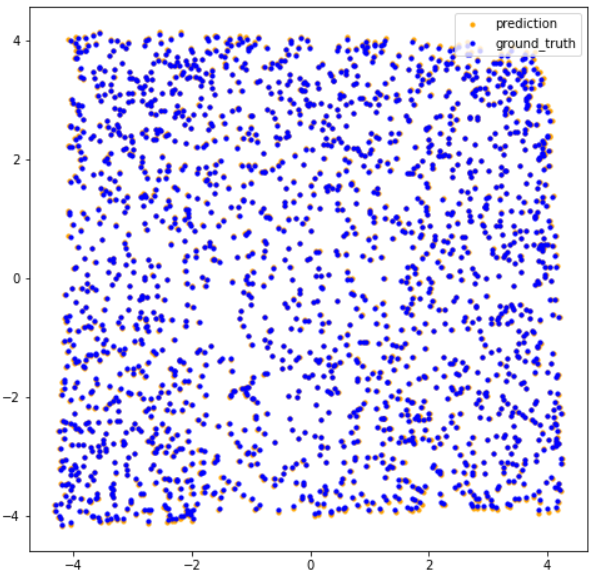
\includegraphics[width=0.34\textwidth]{images/task3-nonlin-final.png}}\\
 \caption{end trajectory points (in orange) against ground truth end points (in blue) - linear vs non linear}%
 \label{fig:task3-linvsnonlin}%
\end{figure}

\paragraph{Part 3}
Eventually, since the results proved the validity of the non linear approximation, we can solve the system starting from all the initial points \texttt{x0} for a much longer time (we opted for \textbf{50}). The non linear vector field shown in \textbf{\hyperref[fig:task3-steadystates]{Figure \ref{fig:task3-steadystates}a}} already shows five apparent steady states, with four of them being close to the corners (\textit{attracting steady states}) and one being near the origin (\textit{repulsive steady state}). Solving the system with \texttt{solve\_ivp} effectively leads to discovering the four attracting steady states, as portrayed in \textbf{\hyperref[fig:task3-steadystates]{Figure \ref{fig:task3-steadystates}b}}. 

To answer the final question, the non linearly approximated system cannot be topologically equivalent to the linearly approximated one because of their different number in steady states, as dynamical systems theory asserts.


\begin{figure}[ht!]
 \centering
 
 \subfloat[a]{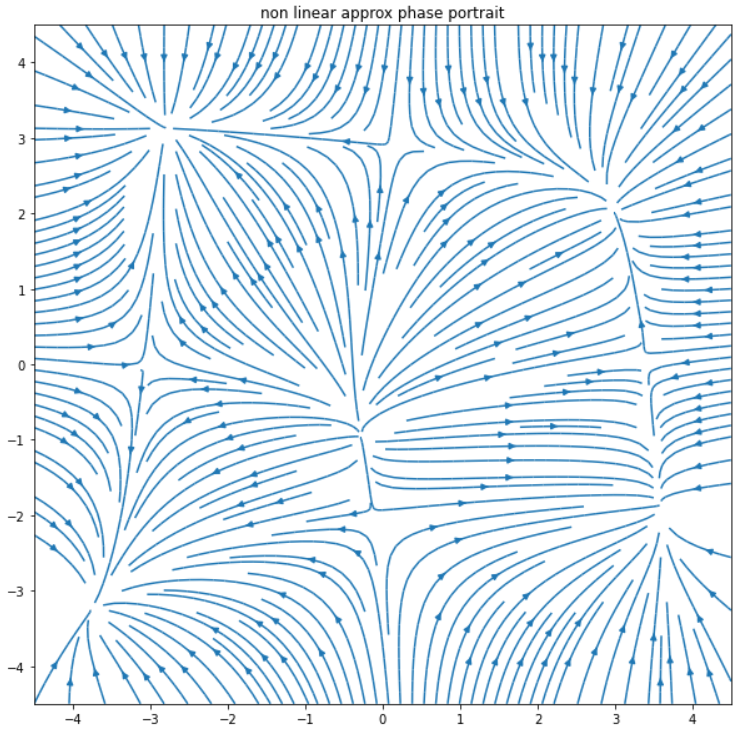
\includegraphics[width=0.4\textwidth]{images/task3-nonlinportrait.png}}%
 \subfloat[b]{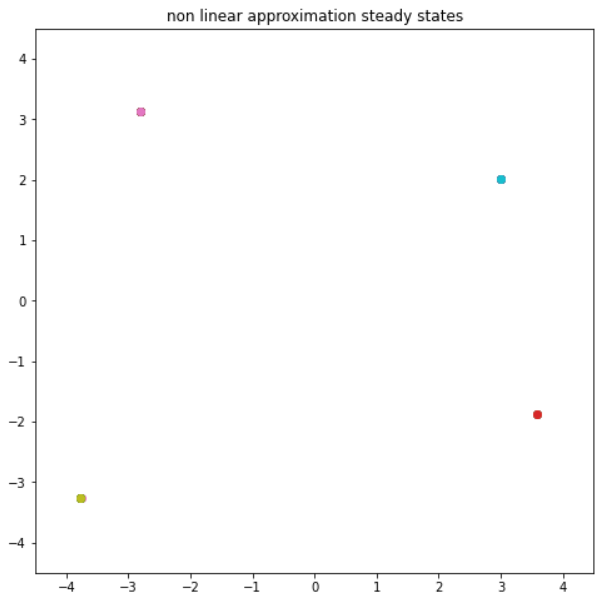
\includegraphics[width=0.41\textwidth]{images/task3-steady-states.png}}
 \caption{best non linear approximation vector field (a) - \textit{attracting} steady states of said vector field (b)}%
 \label{fig:task3-steadystates}%
\end{figure}
\end{task}


\begin{task}{4, Time-delay embedding}
\paragraph{Part 1}
After reading the dataset \texttt{takens\_1.txt}, we plotted the first coordinate against the time (i.e. the line number), obtaining what shown in Figure \hyperref[fig:takens1-coord-1]{\ref{fig:takens1-coord-1}(a)}.
Subsequently, we plotted the same data, but this time not against the line number, but against a delayed version of itself, namely $x(t + \Delta t)$.
Choosing $\Delta t = 10$ (rows), we obtain the result shown in Figure \hyperref[fig:takens1-coord-1]{\ref{fig:takens1-coord-1}(b)}.
According to Takens theorem, being the manifold of dimension $d=1$, it is assured to get an embedding using $2d+1=3$ coordinates, but as it is possible to see in Figure \hyperref[fig:takens1-coord-1]{\ref{fig:takens1-coord-1}(b)}, since there are no intersection in the plot, two coordinates are sufficient to embed this manifold, if a proper time delay is chosen.

\begin{figure}[H]
    \centering
    \subfloat[a]{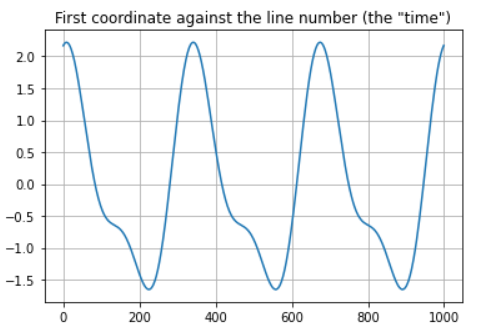
\includegraphics[width=0.45\textwidth]{images/takens1_coord_1.png}}
    \hfill
    \subfloat[b]{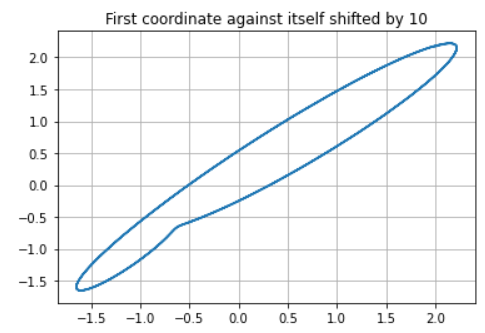
\includegraphics[width=0.45\textwidth]{images/takens1_coord_1_delayed.png}}
    \caption{The first coordinate of the data contained in \texttt{takens\_1.txt} plotted against the time (i.e. the line number) (a) and against a delayed version of itself (b).}
    \label{fig:takens1-coord-1}
\end{figure}

\paragraph{Part 2}
In this part, we test Takens theorem with the chaotic system called the Lorenz attractor. It is shown in Figure \hyperref[fig:lorenz-takens]{\ref{fig:lorenz-takens}(a)}, setting $\sigma = 10,\ \rho = 28,\ \beta = 8/3$ and the starting point equal to $(10,10,10)$.
Now we test Takens theorem by choosing a $\Delta t$ and plotting $x(t)$ against $x(t + \Delta t)$ and $x(t + 2 \Delta t)$, being $x$ the first coordinate of the Lorenz system.
We also try this with the third coordinate: $z$.
The results, with a time delay $\Delta t = 3$ (steps) are shown in Figure \ref{fig:lorenz-takens}.
As it it possible to observe, using the $x$ coordinate we still get a reasonable shape that resembles the original one, while with the $z$ coordinate this does not happen, so the latter is not suitable to represent the original system through a time delay, at least when using two delays ($\Delta t$ and $2 \Delta t$).
This probably happens because for each value of $z$ there are multiple values of the system, and these are found in the two lobes.
In some sense, the two lobes overlap when seen from $z$, and that is why we get a circle-like shape in Figure \hyperref[fig:lorenz-takens]{\ref{fig:lorenz-takens}(c)}.

\begin{figure}[H]
    \centering
    \subfloat[a]{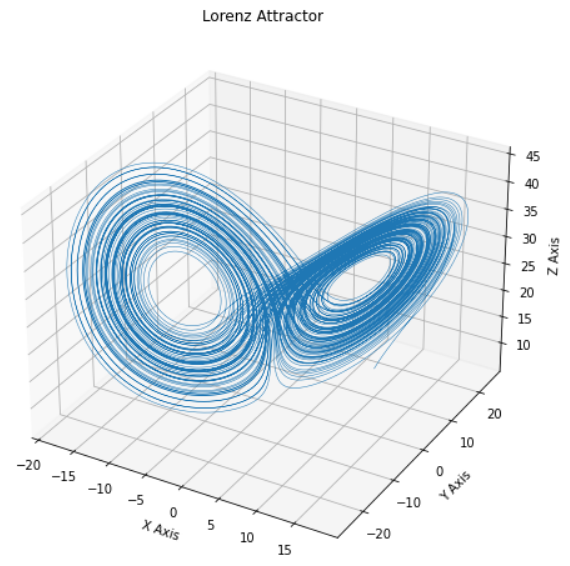
\includegraphics[width=0.45\textwidth]{images/lorenz.png}}\\
    \subfloat[b]{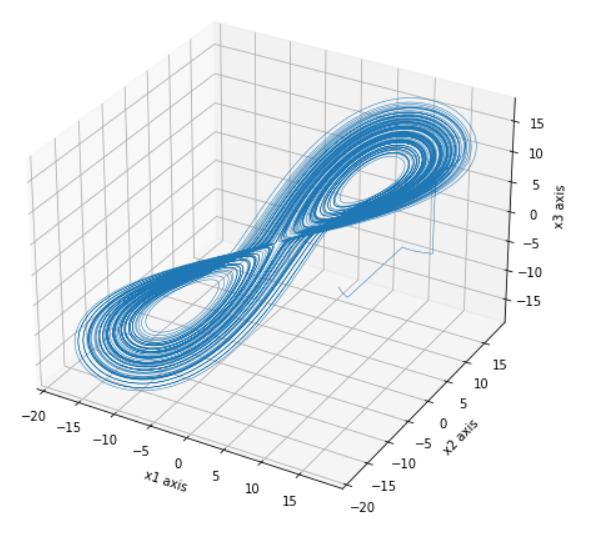
\includegraphics[width=0.45\textwidth]{images/lorenz_takens_x.png}}
    \hfill
    \subfloat[c]{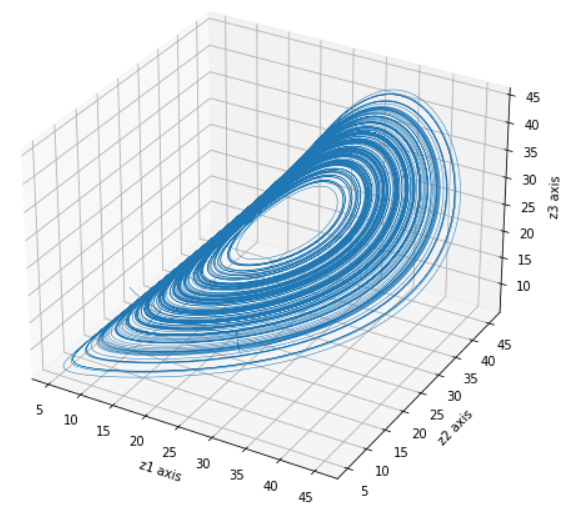
\includegraphics[width=0.45\textwidth]{images/lorenz_takens_z.png}}
    \caption{(a) The Lorenz attractor.
    (b) The Lorenz attractor when plotted using time delays on the $x$ coordinate ($x(t),\ x(t + \Delta t),\ x(t + 2 \Delta t)$.
    (c) The Lorenz attractor when plotted using time delays on the $z$ coordinate ($x(t),\ x(t + \Delta t),\ x(t + 2 \Delta t)$.
    The chosen time delay is 3.}
    \label{fig:lorenz-takens}
\end{figure}

\paragraph{Bonus}
We first created a trajectory concatenating the values of the coordinated $x_1(t) = x(t),\ x_2(t) = x(t + \Delta t),\ x_3(t) = x(t + 2 \Delta t)$.
Then, to compute the approximation through the radial basis functions (using our \texttt{approx\_nonlin\_func} (Fig. \ref{fig:approx-nonlin-func})), we need some points and the corresponding targets.
To get them, we started with our trajectory containing 5000 points\footnote{$[[x(t),\ x(t + \Delta t),\ x(t + 2 \Delta t)]$ for $0 \leq t < 5000]$.}
and used the first 4999 (from the first to the penultimate) as "points" and the second 4999 (from the second to the last) as their "targets".
After approximating the function\footnote{It was easy to obtain good results even approximating the function with a different number of basis functions and/or a different value of $\epsilon$, therefore the values we reported serve simply as an example.}
using 100 bases and $\epsilon=10$, we multiplied the basis functions with the solution matrix from least squares, obtaining a 3-dimensional value for each point in the trajectory.
We proceeded creating a scatter plot of them, obtaining something very similar to the embedding of the attractor with the $x$ coordinate.
The result is shown in Figure \ref{fig:4bonus}

\begin{figure}[H]
    \centering
    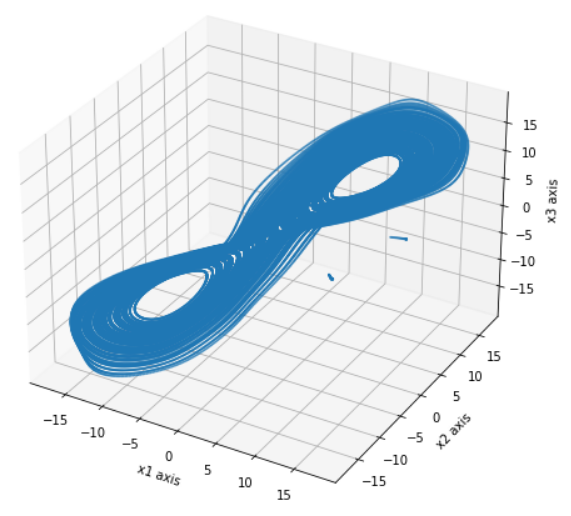
\includegraphics[scale=0.6]{images/4bonus.png}
    \caption{Reconstruction of the $x$ coordinate time delay embedding of the Lorenz attractor after approximating the vector field of the system through a combination of radial basis functions and solving the system.}
    \label{fig:4bonus}
\end{figure}
\end{task}


\begin{task}{5, Learning crowd dynamics}
The last task is centered on learning a dynamical system describing the people flow in nine different areas of TUM Garching, containing the MI Building and the 2 mensas. The given database describes the system over the course of 7 days and is divided as follows: it has a first column containing the \textit{time index} (which is simply a natural number going up one by one and starting from 1) and nine other columns containing the number of people per area at that certain time. In \textbf{\hyperref[fig:task5-data]{Figure \ref{fig:task5-data}}} are therefore shown nine different points at each time step, defining the amount of people per area.
\begin{figure}[H]
    \centering
    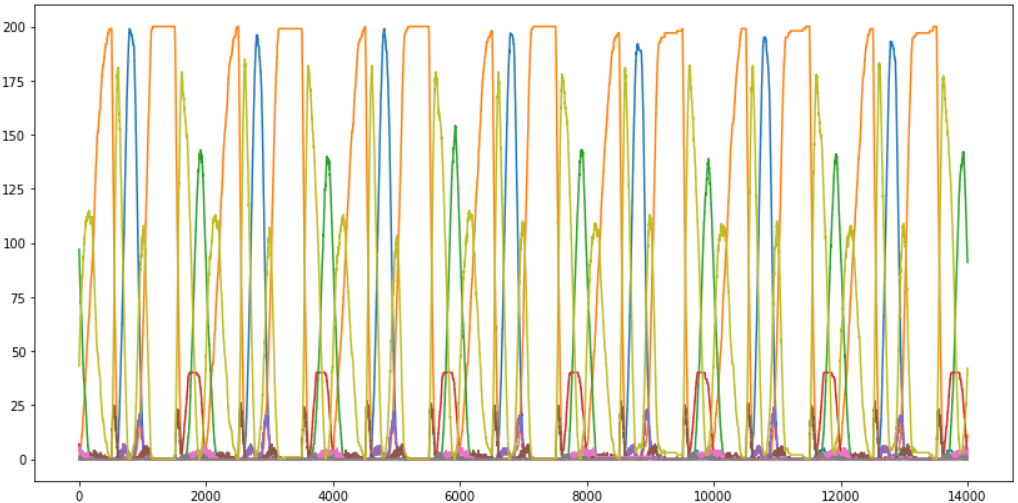
\includegraphics[scale=0.5]{images/task5-data.png}
    \caption{MI building data}
    \label{fig:task5-data}
\end{figure}
\paragraph{Part 1}
The first part of the task hints some important dataset properties, such as it being \textit{periodic} (we know the dataset spans seven days and in fact it is easy to notice how \textbf{\hyperref[fig:task5-data]{Figure \ref{fig:task5-data}}} shows for seven times the same pattern) and with no parametric dependence, therefore being a nine dimensional closed loop which can be reduced to be \textit{one-dimensional}. Following \textbf{Takens theorem}, since we know that \texttt{d=1}, we can assert that it is possible to construct an embedding of the dataset with \texttt{2d+1} dimensions, therefore we need \textbf{three} in order to get a reasonable state space. As a sidenote, first 1000 rows of the dataset have been discarded since they are regarded as \textit{burn-in period} by the exercise sheet.
\begin{figure}[H]
    \centering
    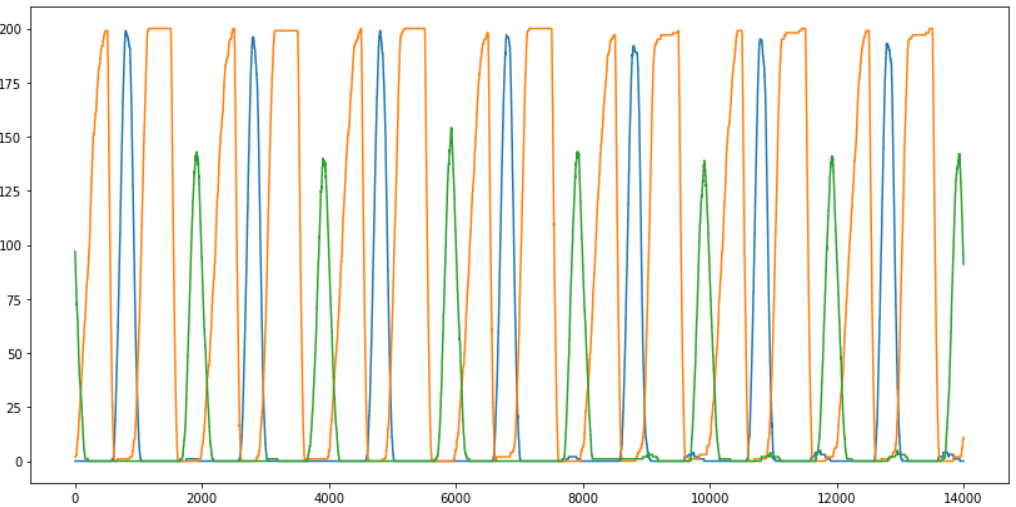
\includegraphics[scale=0.5]{images/task5-data-3.png}
    \caption{MI building data (only first 3 measurements)}
    \label{fig:task5-data-3}
\end{figure}
After reducing the nine measurements zones to three (with the results shown in \textbf{\hyperref[fig:task5-data-3]{Figure \ref{fig:task5-data-3}}}) we create a matrix as required:
\begin{itemize}
    \item each point (row) is a \textit{delay embedding} of the dataset containing only the first three measurements (let us call it \texttt{df}). 
    \item every \textit{delay embedding} is created by taking flattened windows of 351 consecutive 3D points in \texttt{df}.
    \item M of this points are created by moving the start of the delay by one row. We chose M to have maximum possible value, as we have the shape of \texttt{df} and also the length of the window to create a row.
\end{itemize}
Once this rather big \texttt{Mx1053} matrix is created, then we apply PCA to get a matrix maintaining only the \textbf{three} principal components required by Takens, getting the reasonable state space to embed the system, which plot is \textbf{\hyperref[fig:task5-pca-data]{Figure \ref{fig:task5-pca-data}}}.
\begin{figure}[H]
    \centering
    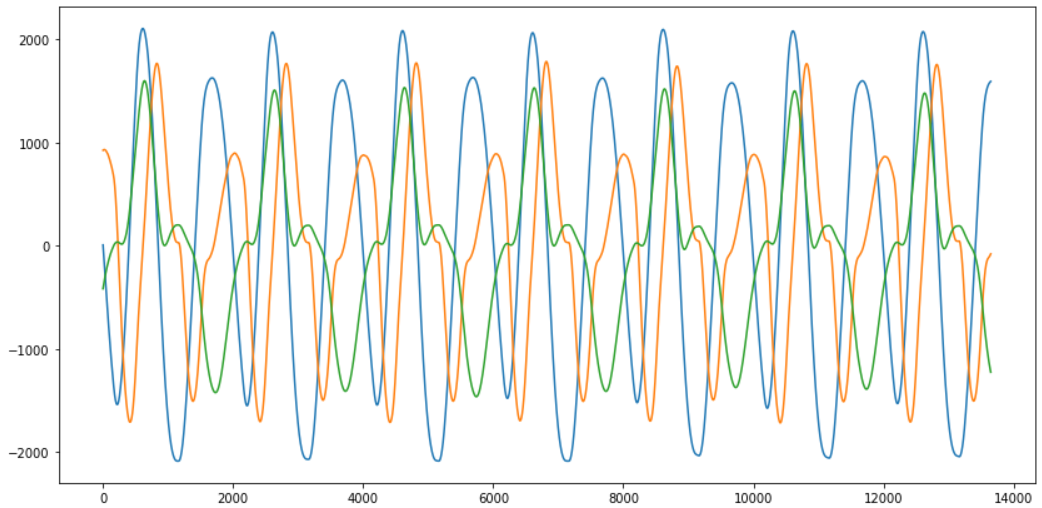
\includegraphics[scale=0.5]{images/task5-pca-data.png}
    \caption{MI building data after PCA dimension reduction to 3 dims}
    \label{fig:task5-pca-data}
\end{figure}

One can appreciate that the reasonable state space is effectively an embedding by visualizing it in 3D (we show it from different angles in \textbf{\hyperref[fig:pca-embedding]{Figure \ref{fig:pca-embedding}}}), where the system shows no intersection. 
\begin{figure}[ht!]
 \centering
 \subfloat{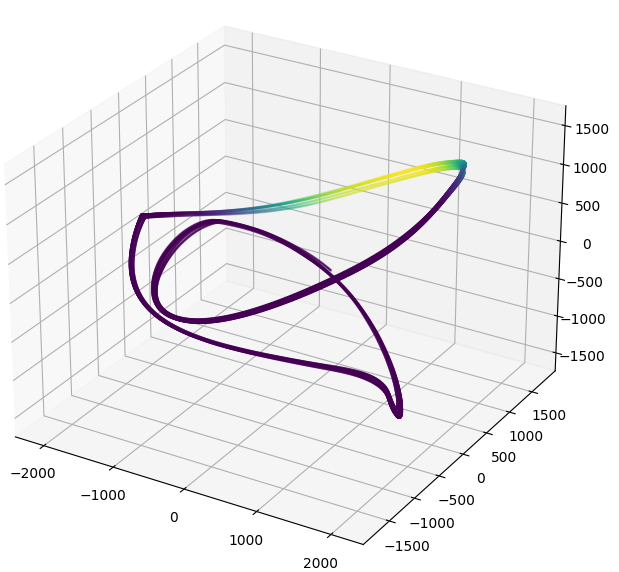
\includegraphics[width=0.34\textwidth]{images/embed_1.png}}%
 \subfloat{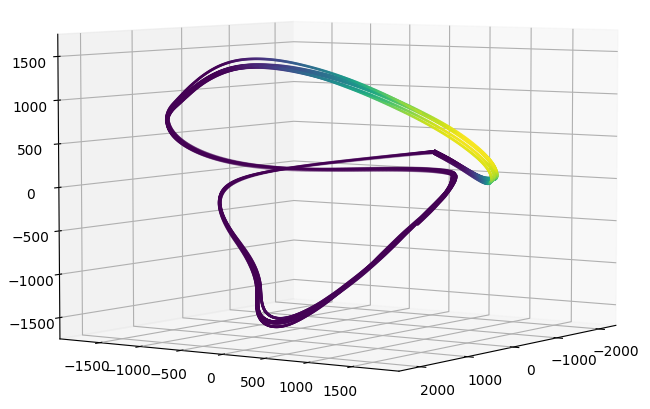
\includegraphics[width=0.34\textwidth]{images/embed_2.png}}%
 \subfloat{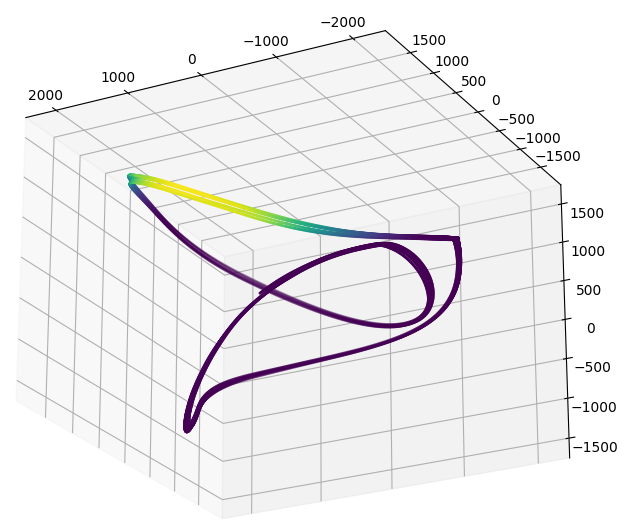
\includegraphics[width=0.34\textwidth]{images/embed_3.png}}\\
 \caption{PCA embedding shown from different angulations}%
 \label{fig:pca-embedding}%
\end{figure}
\pagebreak
\paragraph{Part 2}
We created 9 plots of the PCA embedding coloring the points differently depending on the different measurements areas (i.e. columns) of the original data. These are reported in Figure \ref{fig:task5-part2}.
In order to accomplish this, we simply had to pass the different columns as the color parameter to the \texttt{scatter} function of \texttt{matplotlib}, as shown in Figure \ref{fig:task5-part2-code}.

\begin{figure}[H]
    \centering
    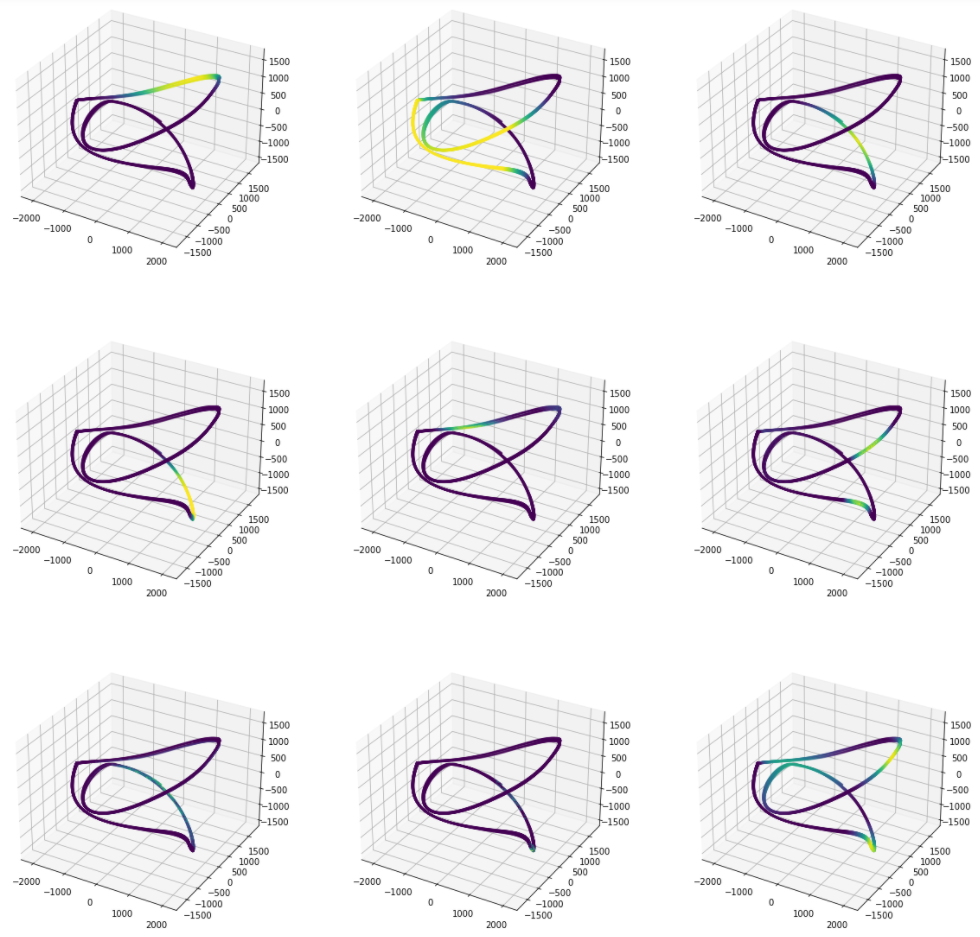
\includegraphics[scale=0.7]{images/task5-part2.png}
    \caption{different measurements coloring on the PCA embedding}
    \label{fig:task5-part2}
\end{figure}

\begin{figure}[H]
    \centering
    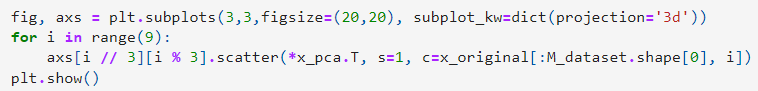
\includegraphics[width=0.8\textwidth]{images/task5-part2-code.png}
    \caption{Function to plot the PCA embedding in different colors depending on the different measurement areas of the original data.}
    \label{fig:my_label}
\end{figure}

\paragraph{Part 3}
Now we are required to learn the dynamics on the curve embedded in the principal components, shown in the previous part. To do so we compute the \textit{arclength} of said curve and approximate its change over time, obtaining therefore the speed of \textit{arclength}, i.e. its first derivative in time, which is a vector field on the \textit{arclength} itself.
To do so we follow these steps:
\begin{itemize}
    \item fixate as first point of the arc the first point in the PCA embedding, beginning of the 3D curve.
    \item iterate through all points (starting from the first point of the arc).
    \item for each couple calculate the \textit{arclength}: accumulate the L2 norm of consecutive points from the first point up to the \texttt{i}-th point.
    \item divide the \textit{arclength} by \texttt{i} (which is the dataset time step, representing also the time passed from starting point to \texttt{i}-th point) to get the speed.
    \item since the data is periodic, cut the vector field to only one period, with result being \textbf{\hyperref[fig:task5-vectorfield]{Figure \ref{fig:task5-vectorfield}}}.
\end{itemize}

\begin{figure}[H]
    \centering
    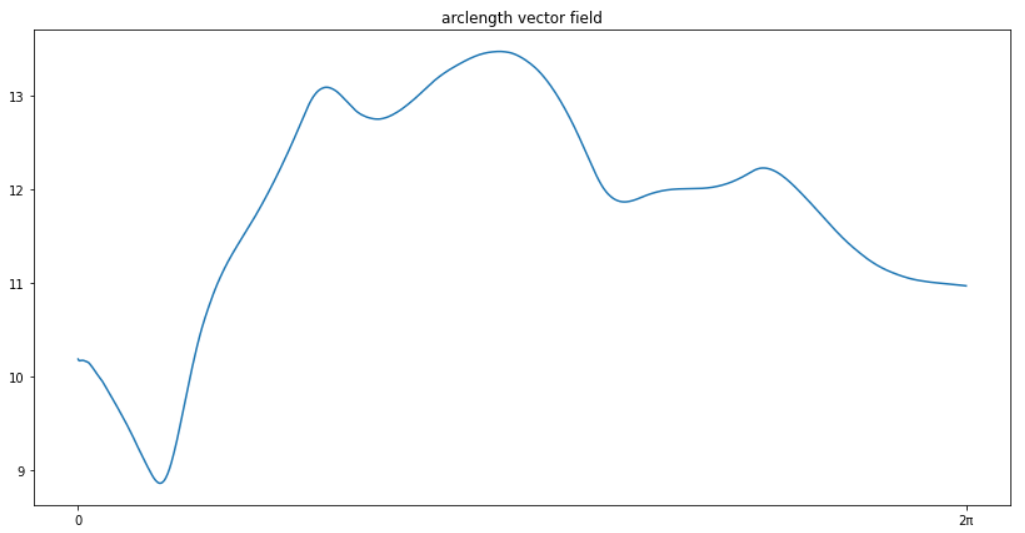
\includegraphics[scale=0.5]{images/task5-vectorfield.png}
    \caption{arclength vector field (one full period)}
    \label{fig:task5-vectorfield}
\end{figure}

To show the periodicity we can observe \textbf{\hyperref[fig:task5-arclen]{Figure \ref{fig:task5-arclen}}}, where the period ending is highlighted by the \textit{red dot}. To find such a period we searched for the nearest point to the starting point (the loop does not exactly pass through the starting point) after a reasonable amount of non-accountable steps. Finding the period let us create such a figure, zeroing the \textit{arclength} accumulation as well as the time passed from the starting point at every period closing.

\begin{figure}[H]
    \centering
    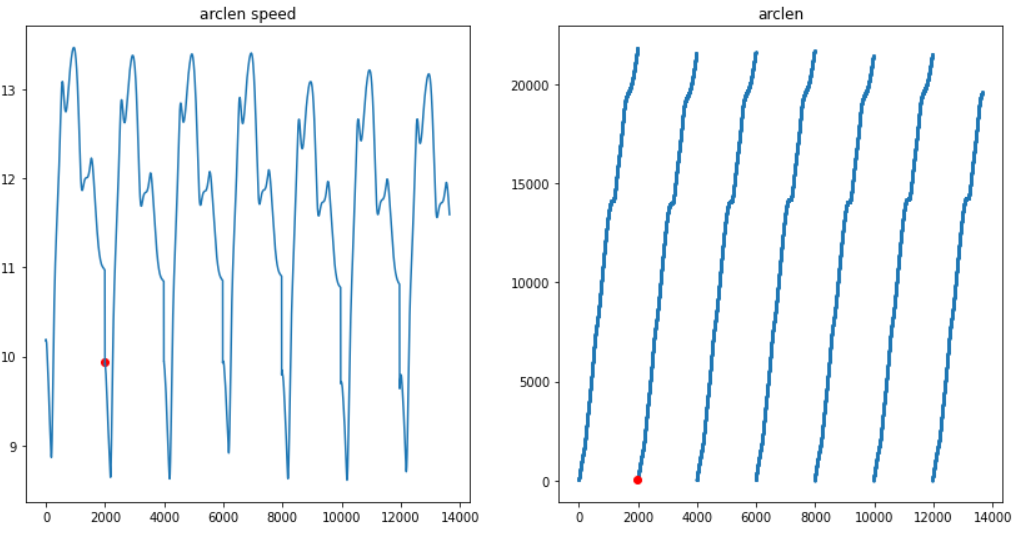
\includegraphics[scale=0.6]{images/task5-arclen.png}
    \caption{seven times repeating arclength vector field (on the left) and arclength (on the right)}
    \label{fig:task5-arclen}
\end{figure}


\paragraph{Part 4}
As last assignment of the sheet we are required to predict the utilization of the MI building for 14 days, hoping the system learns the curve and correctly estimates future unknown points. To do this we start by taking advantage of the \textit{arclength vectorfield} we created in the last part, although we need a way to integrate it for longer time with respect to only a period of one day. To do so we can approximate the \textit{arclength vectorfield} through the aforementioned \textbf{RBF} implementation, treating the arclength data as points and the vectorfield as targets for the least square method. 

\begin{figure}[H]
    \centering
    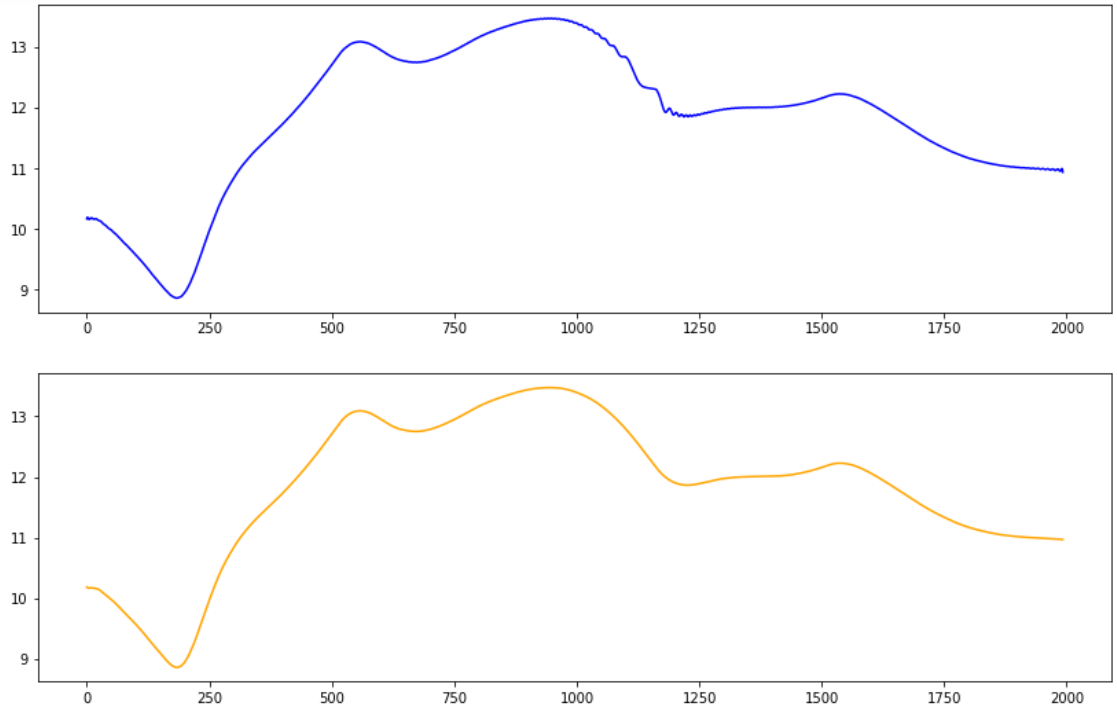
\includegraphics[scale=0.6]{images/task5-rbf-vectorfield.png}
    \caption{rbf approximation of \textit{arclength vector field} (above) vs the groundtruth (below)}
    \label{fig:task5-rbf-vectorfield}
\end{figure}
\textbf{\hyperref[fig:task5-rbf-vectorfield]{Figure \ref{fig:task5-rbf-vectorfield}}} shows the function approximation result. The approximation has been achieved using \texttt{eps = 100} and \texttt{n\_bases = 1000}.

We can continue the path of simulating the MI building utilization by using the \textit{arclength vectorfield} function approximation we just presented, using it to estimate the manifold curve arclength in time. Most importantly we can do so for 14 days, with the results being shown in \textbf{\hyperref[fig:task5-rainbow]{Figure \ref{fig:task5-rainbow}}}.

\begin{figure}[H]
    \centering
    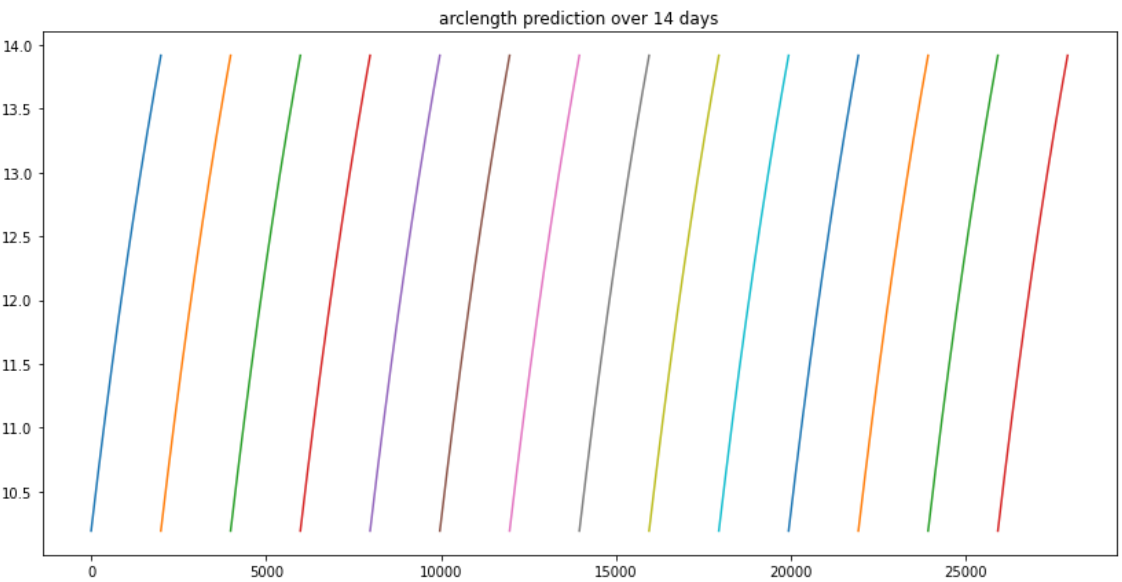
\includegraphics[scale=0.55]{images/task5-rainbow.png}
    \caption{solving the non linearly approximated arclength for 14 days}
    \label{fig:task5-rainbow}
\end{figure}

Once we have the arclength values over time we can map to each arclength the original utilization values since we know how we created them (referring to the time delays) and therefore which arclength corresponds to which utilization value. Having these two paired sets we can construct a radial basis function approximation from arclength space to the utilization value, so we can estimate once again future values. To do so we treat the arclength values as points and the utilization values as targets for the least squares algorithm, effectively finding a function (given by $\Phi C$) which taken an arclength gives the utilization value.
With such a function it is now easy to estimate the utilization value for much longer time, as 14 days, as shown in \textbf{\hyperref[fig:task5-14]{Figure \ref{fig:task5-14}}}.

\begin{figure}[ht!]
 \centering
 \subfloat[a]{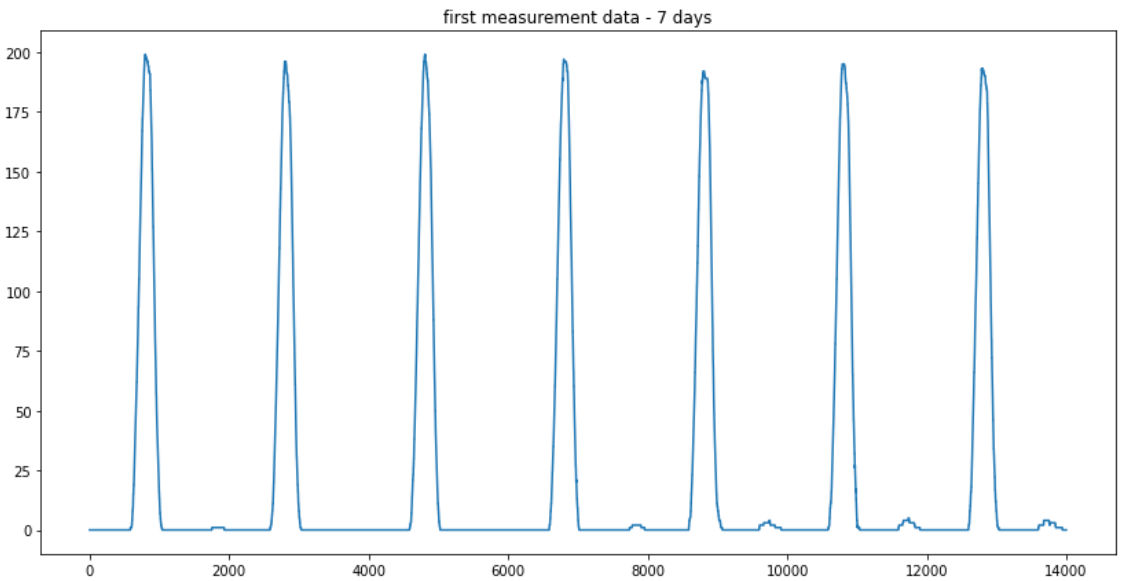
\includegraphics[width=0.6\textwidth]{images/task5-first-measurement.png}}\\
 \subfloat[b]{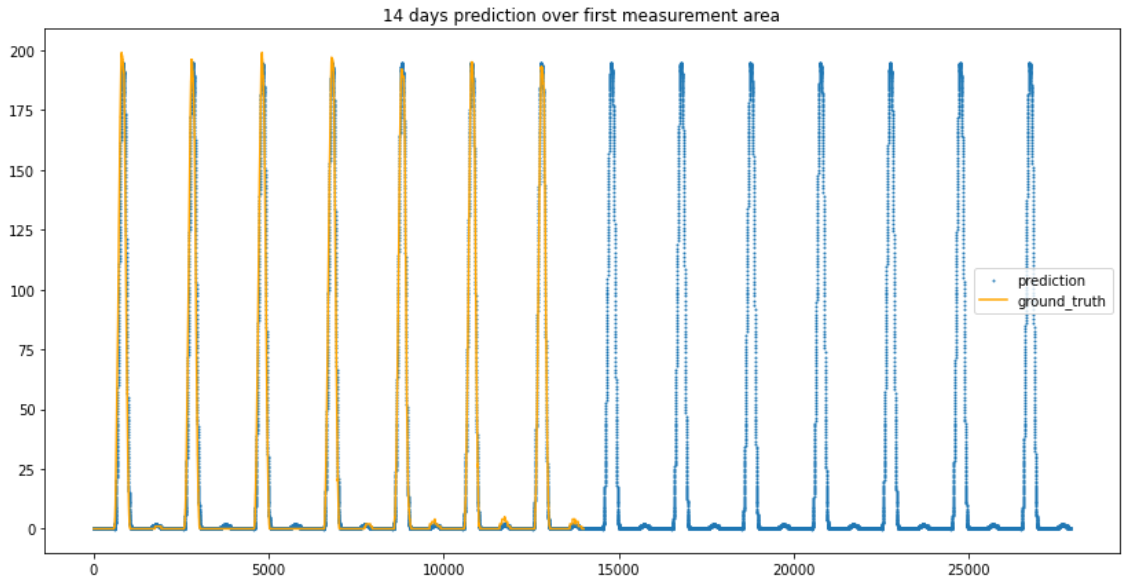
\includegraphics[width=0.6\textwidth]{images/task5-14days.png}}\\
 \caption{MI building utilization ground truth of 7 days (a) and utilization prediction for 14 days (b)}%
 \label{fig:task5-14}%
\end{figure}
\end{task}
\end{document}